\documentclass{article}
\usepackage{graphicx}
\usepackage[utf8]{inputenc}
\usepackage[left=3cm, right=3cm, top=2cm, bottom=2cm]{geometry}
\usepackage{float}
\usepackage[utf8]{inputenc}
\usepackage[polish]{babel}
\usepackage[T1]{fontenc}


\title{Projekt zaliczeniowy}
\author{Wiktor Dybalski, Tomasz Furgała}

\begin{document}

\maketitle
\begin{figure}[H]
    \centering
    
\includegraphics[width=0.7\textwidth]{img/logo.jpg}
    \label{fig:rastrigin}
\end{figure}
\newpage

\section{Cel projektu}
\hspace{0.5cm} Projekt koncentruje się na porównaniu skuteczności dwóch algorytmów minimalizacji stochastycznej: Poszukiwania przypadkowego (PRS) oraz algorytmu wielokrotnego startu (MS). Przeanalizujemy ich wydajność na dwóch różnych funkcjach testowych: funkcji Ackleya i funkcji Rastrigina. Przeprowadzimy porównania dla 2, 10 i 20 wymiarów tych funkcji.

\section{Funkcja Ackley'a}

\hspace{0.5cm} Funkcja Ackleya jest jedną z kluczowych funkcji testowych wykorzystywanych do oceny wydajności algorytmów optymalizacji. Jest to niewypukła funkcja, której minimum globalne znajduje się w centrum przestrzeni poszukiwań. Często stosowana jest jako wyzwanie dla algorytmów, ze względu na swoją złożoność i charakterystyczne lokalne minima.

\[ f(x) = -20 \cdot e^{\left(-0.2 \sqrt{\frac{1}{n} \sum_{i=1}^{n}x_i^2}\right)} - e^{\left(\frac{1}{n} \sum_{i=1}^{n} \cos(2\pi x_i)\right)} + 20 + e
 \]

\begin{figure}[H]
    \centering
    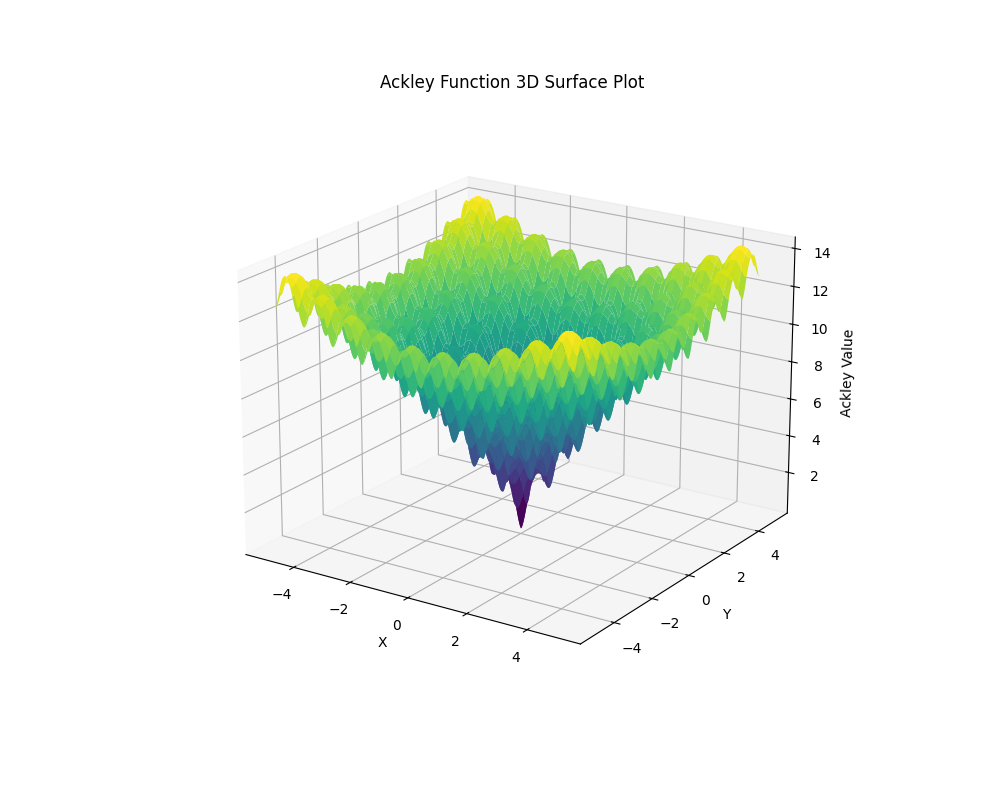
\includegraphics[width=1\textwidth]{img/AckleyFunction.png}
    \label{fig:ackley}
\end{figure}

\newpage

\section{Funkcja Rastrigina}
\hspace{0.5cm}Funkcja Rastrigina to niewypukła funkcja wykorzystywana do testowania wydajności algorytmów optymalizacji. Jej zadaniem jest znalezienie minimum globalnego w przestrzeni n-wymiarowej, gdzie n to liczba zmiennych. Funkcja Rastrigina jest znana ze swoich wielu lokalnych minimów i licznych płaskich obszarów na swojej powierzchni, co sprawia, że jest trudnym wyzwaniem dla algorytmów optymalizacyjnych. Jej wzór jest zdefiniowany jako suma kwadratów wartości zmiennych pomniejszonych o wartość kosinusoidalną, z czym parametr A zwykle wynosi 10.

\[ f(\mathbf{x}) = 10 \cdot n + \sum_{i=1}^{n} \left( x_i^2 - 10 \cdot \cos(2\pi x_i) \right) \]

\begin{figure}[H]
    \centering
    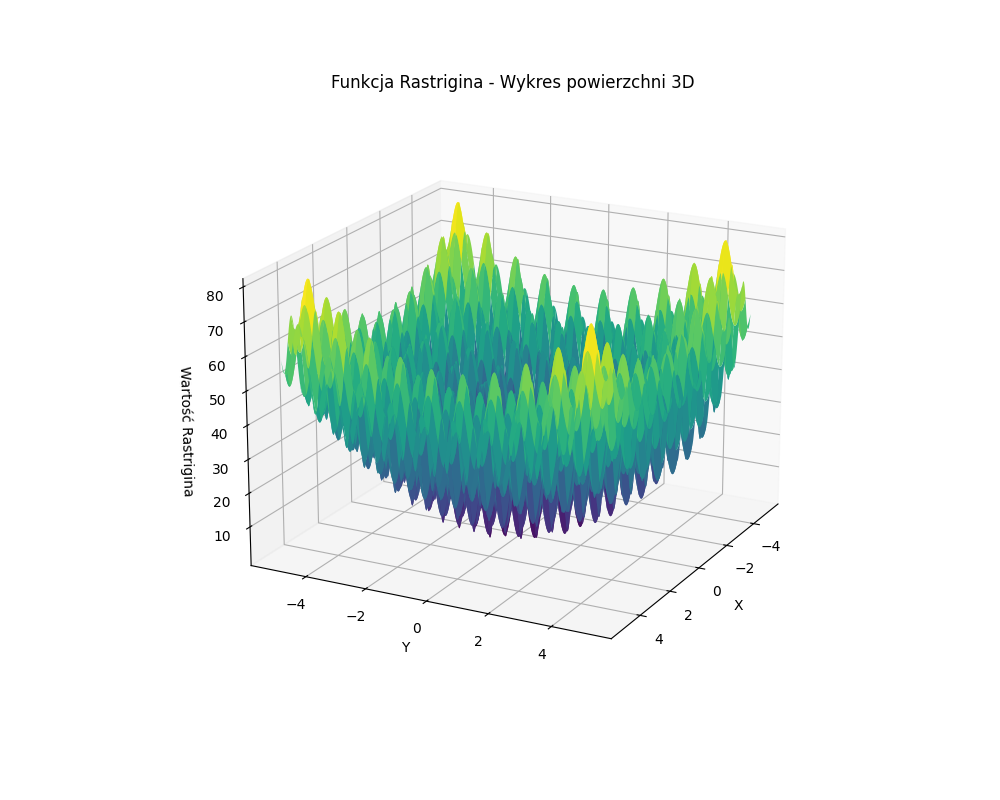
\includegraphics[width=1\textwidth]{img/RastriginFunction.png}
    \label{fig:rastrigin}
\end{figure}

\newpage

\section{Opracowane Wyniki}
\subsection{Funkcja Ackley'a 2d}

\hspace{0.5cm} Algorytm MS znalazł większość puntków w o wartościach w przedziale (0,1). Natomiast kilka punktów znalazło się w przedziale (2,4), zakładamy, że jest to spowodowane większą ilością minimów lokalnych utrudniających znalezienie minima globalnego. Natomiast PRS wypadł dużo gorzej szukając minimum globalnego, znajdując zaledwie kilka punktów o wartościach w przedziale (0,1).

\begin{figure}[H]
    \centering
    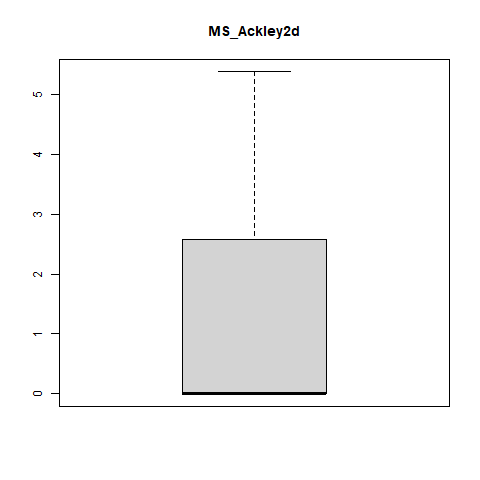
\includegraphics[width=0.55\textwidth]{img/MS_Ackley2d_box.png}
    \label{fig:ackley}
\end{figure}

\begin{figure}[H]
    \centering
    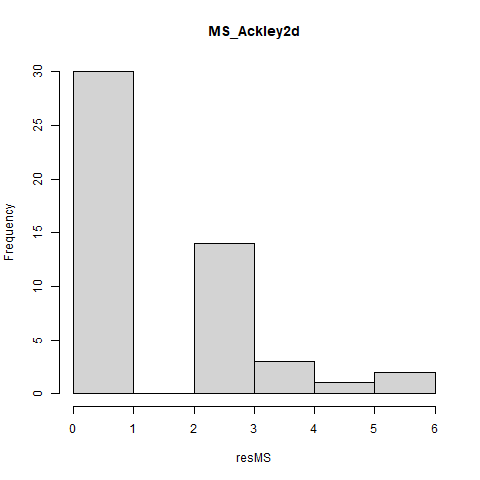
\includegraphics[width=0.55\textwidth]{img/MS_Ackley2d_hist.png}
    \label{fig:ackley}
\end{figure}

\begin{figure}[H]
    \centering
    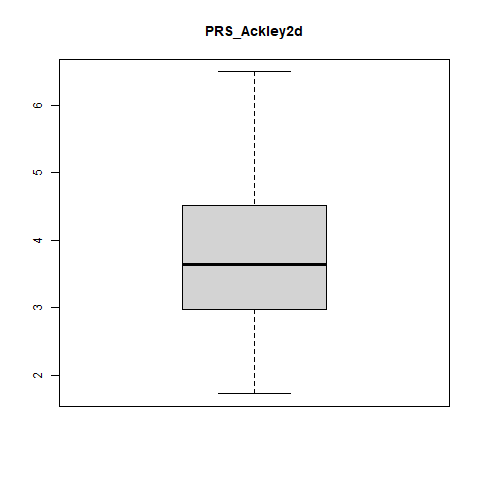
\includegraphics[width=0.55\textwidth]{img/PRS_Ackley2d_box.png}
    \label{fig:ackley}
\end{figure}

\begin{figure}[H]
    \centering
    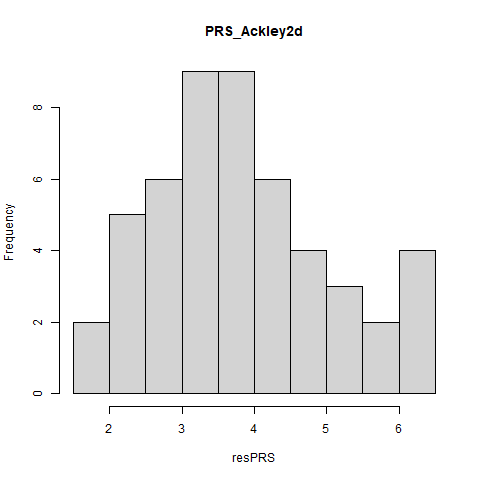
\includegraphics[width=0.55\textwidth]{img/PRS_Ackley2d_hist.png}
    \label{fig:ackley}
\end{figure}



\newpage
\vspace{25pt}
\begin{verbatim}
        One Sample t-test

data:  resMS
t = 5.3204, df = 49, p-value = 2.557e-06
alternative hypothesis: true mean is not equal to 0
95 percent confidence interval:
 0.7777342 1.7218712
sample estimates:
mean of x
 1.249803
\end{verbatim}

\vspace{50pt}

\begin{verbatim}
        One Sample t-test

data:  resPRS
t = 21.752, df = 49, p-value < 2.2e-16
alternative hypothesis: true mean is not equal to 0
95 percent confidence interval:
 3.440863 4.141341
sample estimates:
mean of x
 3.791102
\end{verbatim}

\vspace{50pt}

\begin{verbatim}
        Welch Two Sample t-test

data:  resMS and resPRS
t = -8.6881, df = 90.4, p-value = 1.486e-13
alternative hypothesis: true difference in means is not equal to 0
95 percent confidence interval:
 -3.122372 -1.960227
sample estimates:
mean of x mean of y
 1.249803  3.791102
\end{verbatim}
\newpage

\subsection{Funkcja Ackley'a 10d}

\hspace{0.5cm} Dla 10 wymiarów zauważamy, że obie metody wykazują bardzo podobne wyniki. Średnie wartości pomiarów uzyskane dla obu metod wynoszą około 17,9. Warto zauważyć, że rozbieżność między średnimi wartościami wyznaczonymi przez te metody była minimalna, nie przekraczając 0.1.To pokazuje, że obie metody zwracają bardzo zbliżone rezultaty.  


\begin{figure}[H]
    \centering
    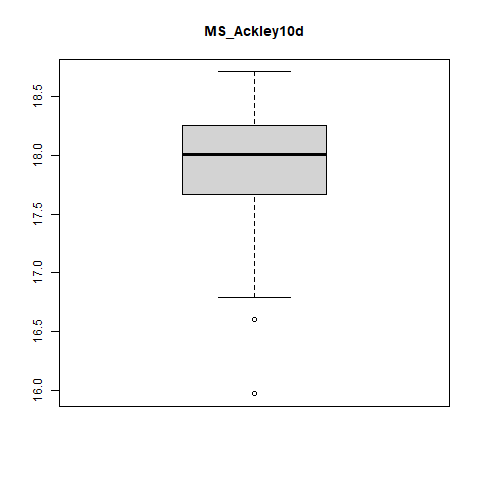
\includegraphics[width=0.55\textwidth]{img/MS_Ackley10d_box.png}
    \label{fig:ackley}
\end{figure}

\begin{figure}[H]
    \centering
    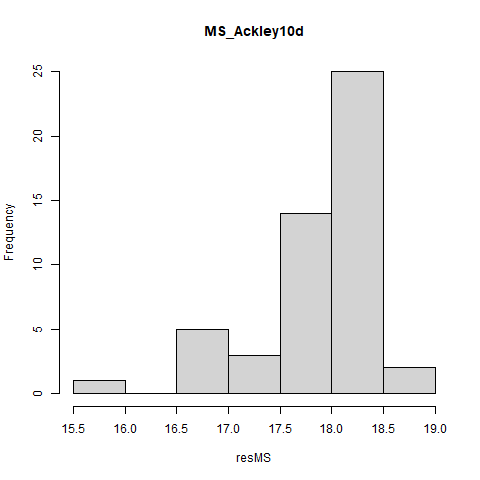
\includegraphics[width=0.55\textwidth]{img/MS_Ackley10d_hist.png}
    \label{fig:ackley}
\end{figure}

\begin{figure}[H]
    \centering
    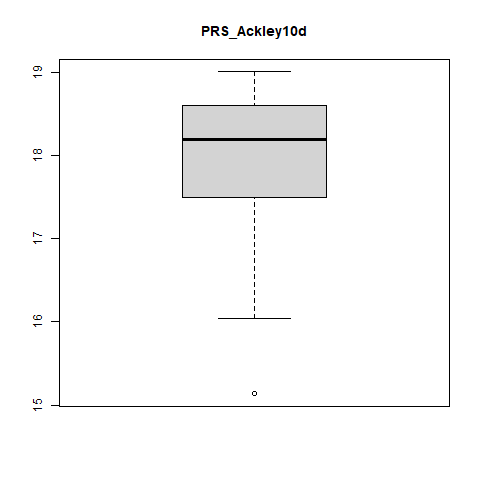
\includegraphics[width=0.55\textwidth]{img/PRS_Ackley10d_box.png}
    \label{fig:ackley}
\end{figure}

\begin{figure}[H]
    \centering
    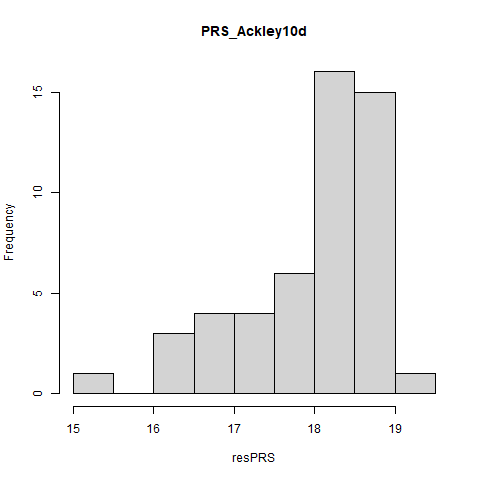
\includegraphics[width=0.55\textwidth]{img/PRS_Ackley10d_hist.png}
    \label{fig:ackley}
\end{figure}

\newpage
\vspace{25pt}

\begin{verbatim}
        One Sample t-test

data:  resMS
t = 223.56, df = 49, p-value < 2.2e-16
alternative hypothesis: true mean is not equal to 0
95 percent confidence interval:
 17.71218 18.03350
sample estimates:
mean of x
 17.87284
\end{verbatim}

\vspace{50pt}

\begin{verbatim}
        One Sample t-test

data:  resPRS
t = 143.94, df = 49, p-value < 2.2e-16
alternative hypothesis: true mean is not equal to 0
95 percent confidence interval:
 17.69124 18.19221
sample estimates:
mean of x
 17.94173
\end{verbatim}

\vspace{50pt}

\begin{verbatim}
        Welch Two Sample t-test

data:  resMS and resPRS
t = -0.4652, df = 83.48, p-value = 0.643
alternative hypothesis: true difference in means is not equal to 0
95 percent confidence interval:
 -0.3633866  0.2256125
sample estimates:
mean of x mean of y
 17.87284  17.94173
\end{verbatim}

\newpage


\subsection{Funkcja Ackley'a 20d}
\hspace{0.5cm} Dla 20 wymiarów, podobnie jak dla 10 wymiarów, obserwujemy, że MS oraz PRS zwracają podobne wyniki, które nie są bliskie 0. Możemy zauważyć także, że dla MS zakres minimów jest znacznie mniejszy niż dla PRS.

\begin{figure}[H]
    \centering
    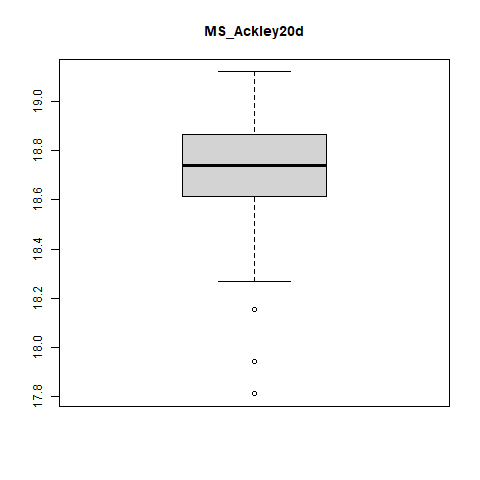
\includegraphics[width=0.55\textwidth]{img/MS_Ackley20d_box.png}
    \label{fig:ackley}
\end{figure}

\begin{figure}[H]
    \centering
    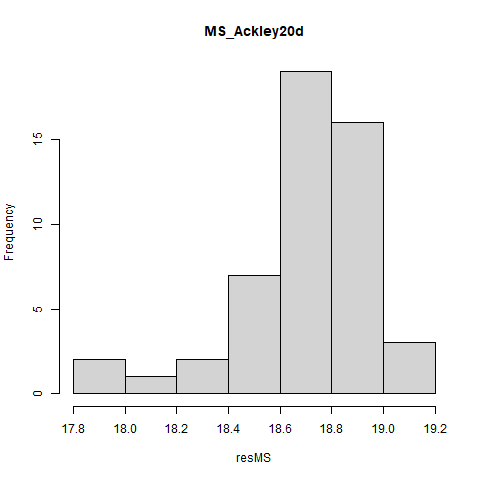
\includegraphics[width=0.55\textwidth]{img/MS_Ackley20d_hist.png}
    \label{fig:ackley}
\end{figure}

\begin{figure}[H]
    \centering
    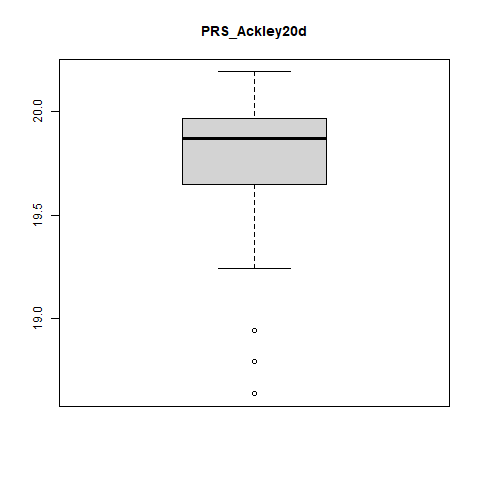
\includegraphics[width=0.55\textwidth]{img/PRS_Ackley20d_box.png}
    \label{fig:ackley}
\end{figure}

\begin{figure}[H]
    \centering
    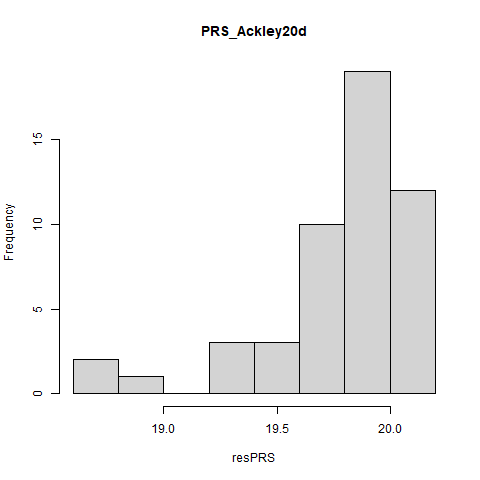
\includegraphics[width=0.55\textwidth]{img/PRS_Ackley20d_hist.png}
    \label{fig:ackley}
\end{figure}

\newpage
\vspace{25pt}

\begin{verbatim}
        One Sample t-test

data:  resMS
t = 505.57, df = 49, p-value < 2.2e-16
alternative hypothesis: true mean is not equal to 0
95 percent confidence interval:
 18.62592 18.77458
sample estimates:
mean of x
 18.70025
\end{verbatim}

\vspace{50pt}

\begin{verbatim}
        One Sample t-test

data:  resPRS
t = 410.94, df = 49, p-value < 2.2e-16
alternative hypothesis: true mean is not equal to 0
95 percent confidence interval:
 19.67672 19.87011
sample estimates:
mean of x
 19.77342
\end{verbatim}

\vspace{50pt}

\begin{verbatim}
        Welch Two Sample t-test

data:  resMS and resPRS
t = -17.682, df = 91.921, p-value < 2.2e-16
alternative hypothesis: true difference in means is not equal to 0
95 percent confidence interval:
 -1.1937083 -0.9526278
sample estimates:
mean of x mean of y
 18.70025  19.77342
\end{verbatim}


\newpage

\subsection{Funkcja Rastrigina 2d}

\hspace{0.5cm} Algorytm MS ponownie znalazł wszystkie punkty w o wartościach w przedziale (0,1).  Natomiast PRS wypadł dużo gorzej szukając minimum globalnego, znajdując zaledwie kilka punktów o wartościach w przedziale (0,1).
\begin{figure}[H]
    \centering
    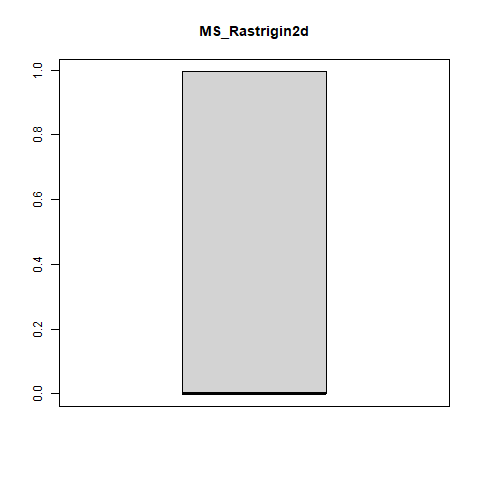
\includegraphics[width=0.55\textwidth]{img/MS_Rastrigin2d_box.png}
    \label{fig:ackley}
\end{figure}

\begin{figure}[H]
    \centering
    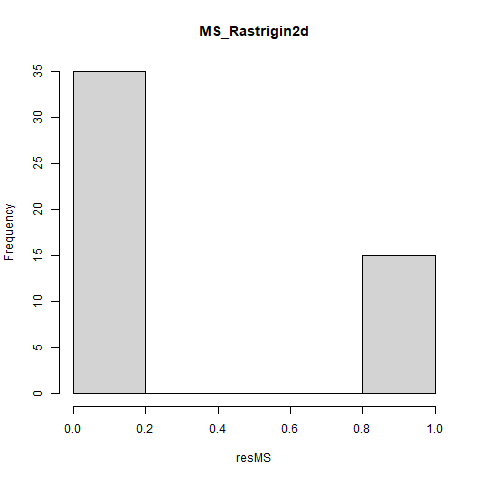
\includegraphics[width=0.55\textwidth]{img/MS_Rastrigin2d_hist.png}
    \label{fig:ackley}
\end{figure}

\begin{figure}[H]
    \centering
    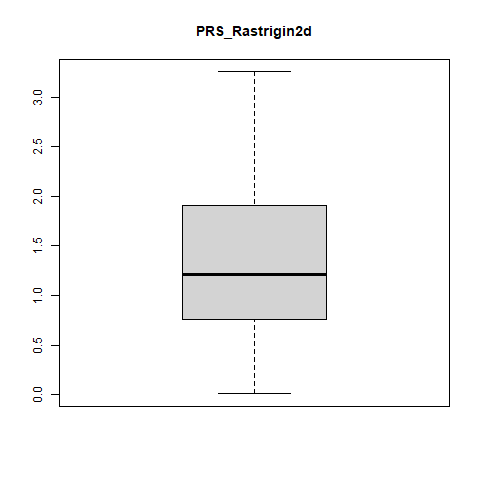
\includegraphics[width=0.55\textwidth]{img/PRS_Rastrigin2d_box.png}
    \label{fig:ackley}
\end{figure}

\begin{figure}[H]
    \centering
    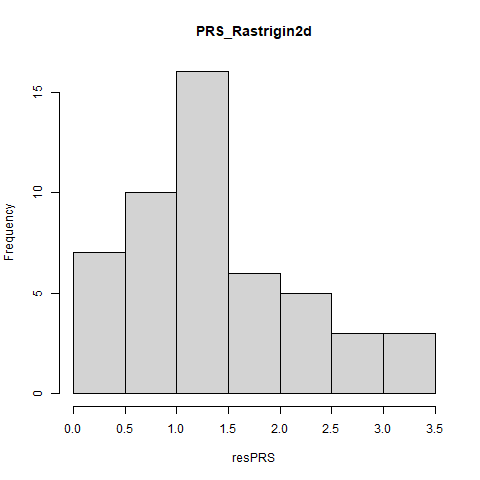
\includegraphics[width=0.55\textwidth]{img/PRS_Rastrigin2d_hist.png}
    \label{fig:ackley}
\end{figure}

\newpage
\vspace{25pt}

\begin{verbatim}
        One Sample t-test

data:  resMS
t = 4.5826, df = 49, p-value = 3.184e-05
alternative hypothesis: true mean is not equal to 0
95 percent confidence interval:
 0.1675933 0.4293821
sample estimates:
mean of x
0.2984877
\end{verbatim}

\vspace{50pt}

\begin{verbatim}
        One Sample t-test

data:  resPRS
t = 11.339, df = 49, p-value = 2.641e-15
alternative hypothesis: true mean is not equal to 0
95 percent confidence interval:
 1.125987 1.611071
sample estimates:
mean of x
 1.368529
\end{verbatim}

\vspace{50pt}

\begin{verbatim}
        Welch Two Sample t-test

data:  resMS and resPRS
t = -7.8021, df = 75.311, p-value = 2.771e-11
alternative hypothesis: true difference in means is not equal to 0
95 percent confidence interval:
 -1.3432345 -0.7968479
sample estimates:
mean of x mean of y 
0.2984877 1.3685289

\end{verbatim}


\newpage

\subsection{Funkcja Rastrigina 10d} 

\hspace{0.5cm} Dla 10 wymiarów żadna z metod nie zwraca wartości zbliżoneych do 0, natomiast rezultaty metody MS są znacznie lepsze w porównaniu do PRS.

\begin{figure}[H]
    \centering
    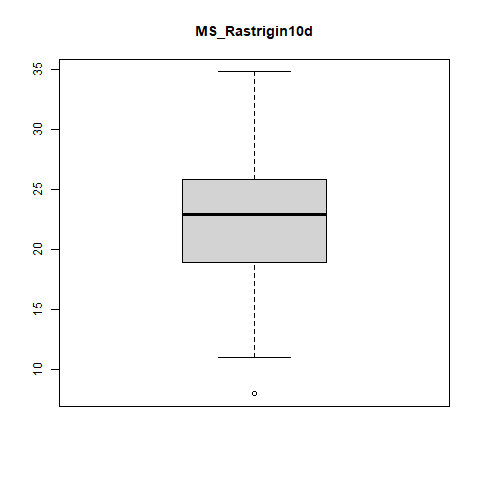
\includegraphics[width=0.55\textwidth]{img/MS_Rastrigin10d_box.png}
    \label{fig:ackley}
\end{figure}

\begin{figure}[H]
    \centering
    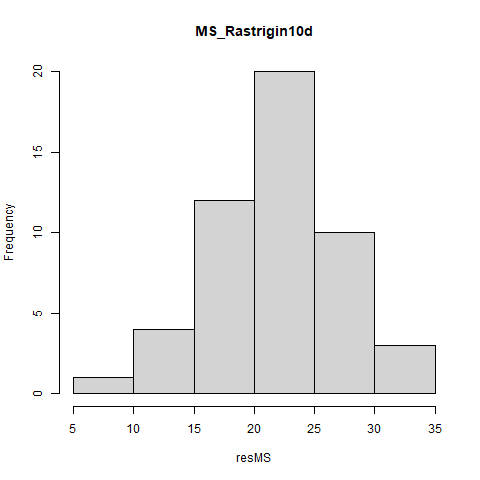
\includegraphics[width=0.55\textwidth]{img/MS_Rastrigin10d_hist.png}
    \label{fig:ackley}
\end{figure}

\begin{figure}[H]
    \centering
    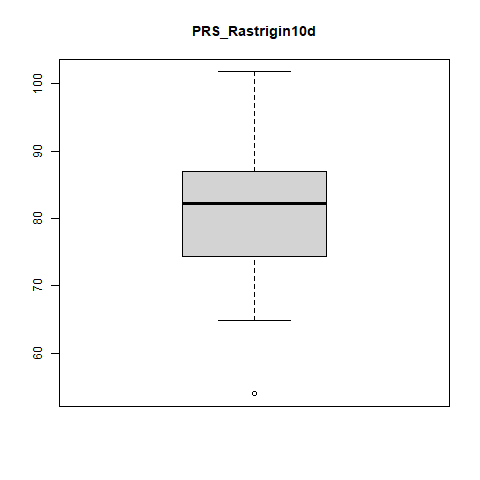
\includegraphics[width=0.55\textwidth]{img/PRS_Rastrigin10d_box.png}
    \label{fig:ackley}
\end{figure}

\begin{figure}[H]
    \centering
    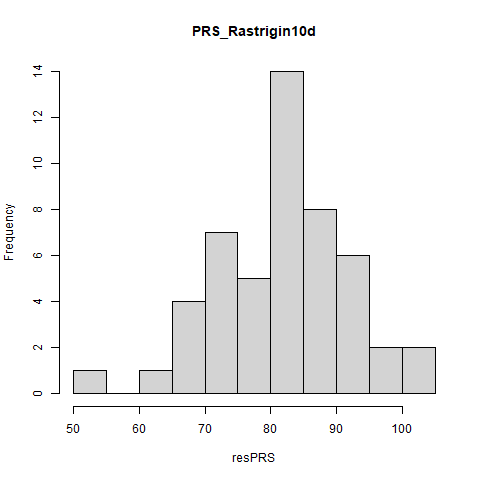
\includegraphics[width=0.55\textwidth]{img/PRS_Rastrigin10d_hist.png}
    \label{fig:ackley}
\end{figure}

\newpage
\vspace{25pt}

\begin{verbatim}
        One Sample t-test

data:  resMS
t = 28.964, df = 49, p-value < 2.2e-16
alternative hypothesis: true mean is not equal to 0
95 percent confidence interval:
 20.83330 23.93976
sample estimates:
mean of x
 22.38653
\end{verbatim}

\vspace{50pt}

\begin{verbatim}
        One Sample t-test

data:  resPRS
t = 60.738, df = 49, p-value < 2.2e-16
alternative hypothesis: true mean is not equal to 0
95 percent confidence interval:
 78.85508 84.25164
sample estimates:
mean of x
 81.55336
\end{verbatim}

\vspace{50pt}

\begin{verbatim}
        Welch Two Sample t-test

data:  resMS and resPRS
t = -38.19, df = 78.26, p-value < 2.2e-16
alternative hypothesis: true difference in means is not equal to 0
95 percent confidence interval:
 -62.25105 -56.08261
sample estimates:
mean of x mean of y
 22.38653  81.55336

\end{verbatim}


\newpage

\subsection{Funkcja Rastrigina 20d}

\hspace{0.5cm} Podobnie jak dla 10 wymiarów, dla 20, żadna z metod nie zwraca wartości zbliżonych do 0, natomiast rezultaty metody MS są znacznie lepsze w porównaniu do PRS.

\begin{figure}[H]
    \centering
    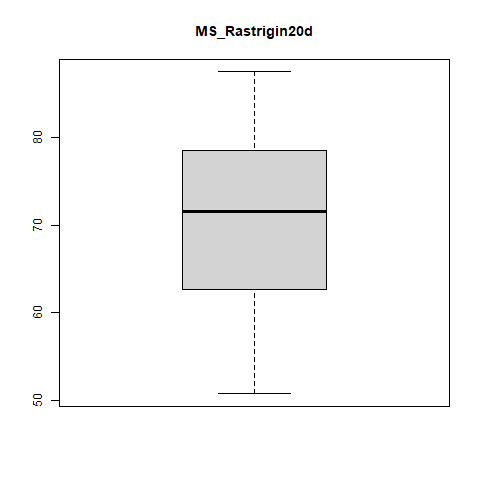
\includegraphics[width=0.55\textwidth]{img/MS_Rastrigin20d_box.png}
    \label{fig:ackley}
\end{figure}

\begin{figure}[H]
    \centering
    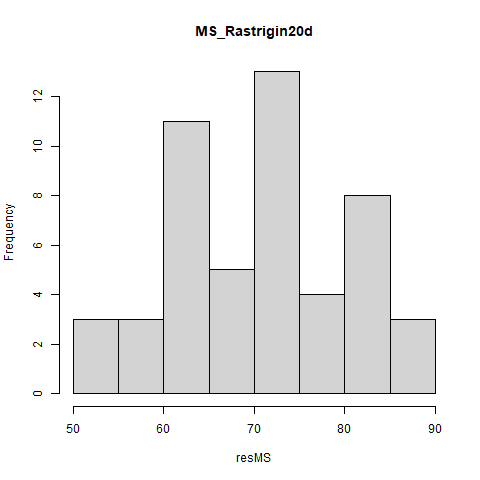
\includegraphics[width=0.55\textwidth]{img/MS_Rastrigin20d_hist.png}
    \label{fig:ackley}
\end{figure}

\begin{figure}[H]
    \centering
    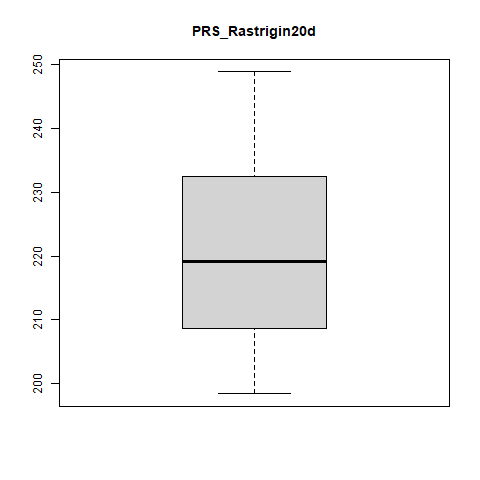
\includegraphics[width=0.55\textwidth]{img/PRS_Rastrigin20d_box.png}
    \label{fig:ackley}
\end{figure}

\begin{figure}[H]
    \centering
    \label{fig:ackley}
\end{figure}

\newpage
\vspace{25pt}

\begin{verbatim}
        One Sample t-test

data:  resMS
t = 51.94, df = 49, p-value < 2.2e-16
alternative hypothesis: true mean is not equal to 0
95 percent confidence interval:
 67.83219 73.29229
sample estimates:
mean of x
 70.56224
\end{verbatim}

\vspace{50pt}

\begin{verbatim}
        One Sample t-test

data:  resPRS
t = 119, df = 49, p-value < 2.2e-16
alternative hypothesis: true mean is not equal to 0
95 percent confidence interval:
 216.5235 223.9619
sample estimates:
mean of x
 220.2427
\end{verbatim}

\vspace{50pt}

\begin{verbatim}
        Welch Two Sample t-test

data:  resMS and resPRS
t = -65.197, df = 89.923, p-value < 2.2e-16
alternative hypothesis: true difference in means is not equal to 0
95 percent confidence interval:
 -154.2415 -145.1194
sample estimates:
mean of x mean of y
 70.56224 220.24269

\end{verbatim}


\newpage

\section{Wnioski}

\hspace{0.5cm} Z wyników obliczeń wyraźnie wynika, że algorytm MS wykazuje przewagę nad algorytmem PRS w kontekście efektywnego znajdowania minimów. Algorytm MS, który korzysta z funkcji "optim" z metodą L-BFGS-B, demonstruje znacznie lepszą skuteczność. Jednym z kluczowych czynników przyczyniających się do tego sukcesu jest fakt, że algorytm MS nie polega na losowaniu punktów do sprawdzenia, ale wykorzystuje gradient funkcji. Dzięki temu jest w stanie lepiej przewidzieć, w którą stronę powinien podążać w procesie optymalizacji, co skutkuje bardziej efektywnym znajdowaniem odpowiednich minimów.



\section{Implementacje}
\subsection{Pure Random Search, PRS}

\hspace{0.5cm} Funkcja PRS implementuje algorytm losowego przeszukiwania w celu minimalizacji funkcji celu. Generuje ona losowe punkty w przestrzeni poszukiwań i ocenia ich wartość, zwracając najmniejszą znalezioną wartość. Jest to prosty, ale nieefektywny sposób eksploracji przestrzeni poszukiwań, który może być przydatny do szybkiego zrozumienia ogólnej struktury funkcji celu, zwłaszcza w wysokowymiarowych problemach optymalizacyjnych.

\begin{verbatim}
PRS <- function(fun, num_of_points, dim){
  min_value <- Inf
  for(x in 1:num_of_points){
    point <- runif(dim, getLowerBoxConstraints(fun), getUpperBoxConstraints(fun))
    value <- fun(point)

    if(value < min_value){
      min_value <- value
    }
  }
  return(min_value)
}
\end{verbatim}




\subsection{Multi-start, MS}

\hspace{0.5cm} Funkcja MS implementuje algorytm wielokrotnego startu w celu minimalizacji funkcji celu. W każdej iteracji generuje losowy punkt w przestrzeni poszukiwań, a następnie stosuje algorytm optymalizacji lokalnej (np. L-BFGS-B) z tego punktu startowego. Zwraca najmniejszą znalezioną wartość funkcji celu oraz całkowitą liczbę wywołań algorytmu optymalizacji lokalnej.

\begin{verbatim}
MS <- function(fun, num_points, dim) {
  min_values <- Inf
  total_MS_calls <- 0

  for (i in 1:num_points) {
    point <- runif(dim, getLowerBoxConstraints(fun), getUpperBoxConstraints(fun))
    result <- optim(par = point, fn = fun, method = "L-BFGS-B" , 
                        lower = getLowerBoxConstraints(fun), 
                        upper = getUpperBoxConstraints(fun))
    value <- result$value
    total_MS_calls <- total_MS_calls + result$counts[1]  

    min_values[i] <- value
  }
  return(list(min(min_values),total_MS_calls))
}
\end{verbatim}



\subsection{Main function}

\hspace{0.5cm} Poniższy kod to funkcja main, która przeprowadza analizę porównawczą algorytmów minimalizacji stochastycznej (MS i PRS) na funkcji Ackleya o dwóch wymiarach. Funkcja generuje wyniki dla 50 replikacji obu algorytmów, a następnie tworzy histogramy i boxploty dla wyników MS i PRS. Dodatkowo przeprowadza testy t dla obu algorytmów oraz dla wyników obu algorytmów. Dla kolejnych porówniań zmieniamy ilość wymiarów oraz wykorzystywaną funkcje.

\begin{verbatim}
main <- function() {
  dim <- 2
  num_points <- 100
  ackley_function <- makeAckleyFunction(dimensions = dim)
  
  resMSlist <- replicate(50, MS(ackley_function, num_points, dim))
  resMS <- as.numeric(resMSlist[1,])  
  points <- as.numeric(resMSlist[2,])  

  resPRS <- replicate(50, PRS(ackley_function, mean(points), dim))
  
    png("MS_Ackley2d_hist.png")
    hist(resMS, main = "MS_Ackley2d")
    dev.off() 
    png("MS_Ackley2d_box.png")
    boxplot(resMS, main = "MS_Ackley2d")
    dev.off()

    png("PRS_Ackley2d_hist.png")
    hist(resPRS, main = "PRS_Ackley2d")
    dev.off()

    png("PRS_Ackley2d_box.png")
    boxplot(resPRS, main = "PRS_Ackley2d")
    dev.off()

    testMS <- t.test(resMS, mu=0)
    print(testMS)

    testPRS <- t.test(resPRS, mu=0)
    print(testPRS)

    testBoth <- t.test(resMS, resPRS, mu=0)

    print(testBoth)
}   

\end{verbatim}


\end{document}

